\section{Понятие о скалярных, векторных и тензорных величинах}

\subsection{Скаляры}

    Скаляр -- физическая или математическая величина, которая описывается числом или функцией. Скаляр инвариантен относительно преобразований координат. Примерами скаляров являются
    \begin{itemize}
        \item масса \( m \); 
        \item потенциал \( \phi = \phi(x, y, z) \);
        \item работа \( A \);
        \item температура \( T = T(x, y, z, t) \);
        \item давление \( P = P(x, y, z, t) \).
    \end{itemize}

subsection{Векторы}

    Вектор, в отличие от скаляра, характеризуется не одним, а тремя независимыми числами:
    \[ \vec{a} = \{ a_{x}, a_{y}, a_{z} \}. \]

    Однако, не все тройки чисел являются векторами. Так например вектором не является тройка \( (P,\ V,\ T) \), так как одна из величин связана с двумя другими при помощи уравнения состояния.
    
    Векторами являются такие физические величины, как
    \begin{itemize}
        \item скорость \( \vec{v} = \{v_x(x, y, z),\ v_y(x, y, z),\ v_z(x, y, z)\} \);
        \item сила \( \vec{F} = \{F_x(x, y, z),\ F_y(x, y, z),\ F_z(x, y, z)\} \);
        \item напряжённость электрического поля \( \vec{E} = \vec{E}(x, y, z) \).
    \end{itemize}

\subsection{Тензоры}

    Тензор является более общим понятием, чем скаляр. Тензор, в зависимости от своего ранга, характеризуется \( 3^n \) числами. Для нас тензор будет характеризоваться \( 3^2 \), \( 3^3 \) и \( 3^4 \) числами.
    
    Тензоры появляются в ситуациях, когда требуется описать какое-либо явление, происходящее в неоднородной среде. Рассмотрим для примера закон Ома.
    
    Если среда изотропна, то закон Ома имеет вид \( i = \frac{1}{R} U \).
    
    Запишем его в дифференциальном виде:
    \[ \vec{j} = \lambda \vec{E} \]
    или в проекциях: 
    \begin{equation}
    \left\{ \begin{array}{l}
            j_{1} = \lambda E_{1}, \\
            j_{2} = \lambda E_{2}, \\
            j_{3} = \lambda E_{3};
    \end{array} \right. \label{eq1.1}
    \end{equation}
    где \( \vec{j} \) -- плотность тока, \( \vec{E} \) -- электрическое поле, \( \lambda \) -- удельная проводимость материала (скалярная величина),

    В этом случае вектор \( \vec{j} \) сонаправлен вектору \( \vec{E} \).

    Если среда анизотропна, то вместо (\ref{eq1.1}) надо записать следующее:
    \begin{equation}
        \left\{
        \begin{array}{c}
            j_{1} = \lambda_{11} E_{1} + \lambda_{12} E_{2} + \lambda_{13} E_{3}, \\
            j_{2} = \lambda_{21} E_{1} + \lambda_{22} E_{2} + \lambda_{23} E_{3}, \\
            j_{3} = \lambda_{31} E_{1} + \lambda_{32} E_{2} + \lambda_{33} E_{3}
        \end{array}
        \right.
    \end{equation}
    или 
    \[ j_{k} = \sum\limits_{i=1}^3 \lambda_{ki} E_i, \]
    где \( k = 1,\ 2,\ 3 \).
    
    В матричном виде это будет выглядеть так:
    \[ \vec{j} = \Lambda \vec{E}, \]
    где \( \Lambda \) -- матрица тензора электропроводимости:
    \[ \Lambda =
        \begin{pmatrix}
            \lambda_{11} & \lambda_{12} & \lambda_{13} \\
            \lambda_{21} & \lambda_{22} & \lambda_{23} \\
            \lambda_{31} & \lambda_{32} & \lambda_{33} 
        \end{pmatrix}. \]

    Поэтому в общем случае вектор \( \vec{j} \) неколлинеарен вектору \( \vec{E} \).

    \begin{definition}
        Cреда называется линейной, если её реакция \( y \) связана каким-либо линейным соотношением с воздействием \( X \): \( y = L(X) \).
    \end{definition}
 
    В линейных среда выполняется все линейные законы:
    \begin{itemize}
        \item закон Ома \( i = u/r \), для анизотропной среды: \( \vec{j} = \Lambda \vec{E} \);
        \item закон Гука \( \sigma = \eps E \);
        \item закон Фурье \( \vec{j} = -k \nabla T \).
    \end{itemize}

    Если \( \vec{j} \sim E^2 \), то говорят, что среда нелинейна относительно поля \( \vec{E} \). 

    Пример нелинейных сред:
    \begin{itemize}
        \item ферромагнетики - типичные нелинейные среды, т.к. в них \( \vec{B} \nsim \vec{H} \);
        \item сегнетоэлектрики.
    \end{itemize}
 
    \begin{definition}
        Среда называется однородной, если её свойства одинаковы во всех точках. В противном случае среда называется неоднородной.
    \end{definition}

    \begin{definition}
        Среда называется изотропной, если её свойства в данной точке одинаковы по всем направлениям. В противном случае среда называется анизотропной.
    \end{definition}

    Если предметом векторной алгебры являются алгебраические операции с постоянными векторами, то предметом векторного анализа являются свойства и операции над скалярными и векторными полями, определённые в трехмерном евклидовом пространстве.

\subsection{Понятие об инвариантности свойств объектов}

    Рассмотрим вектор \( \vec{a} = \{a_x, a_y, a_z\} \):
    \begin{figure}[ht]
        \center
        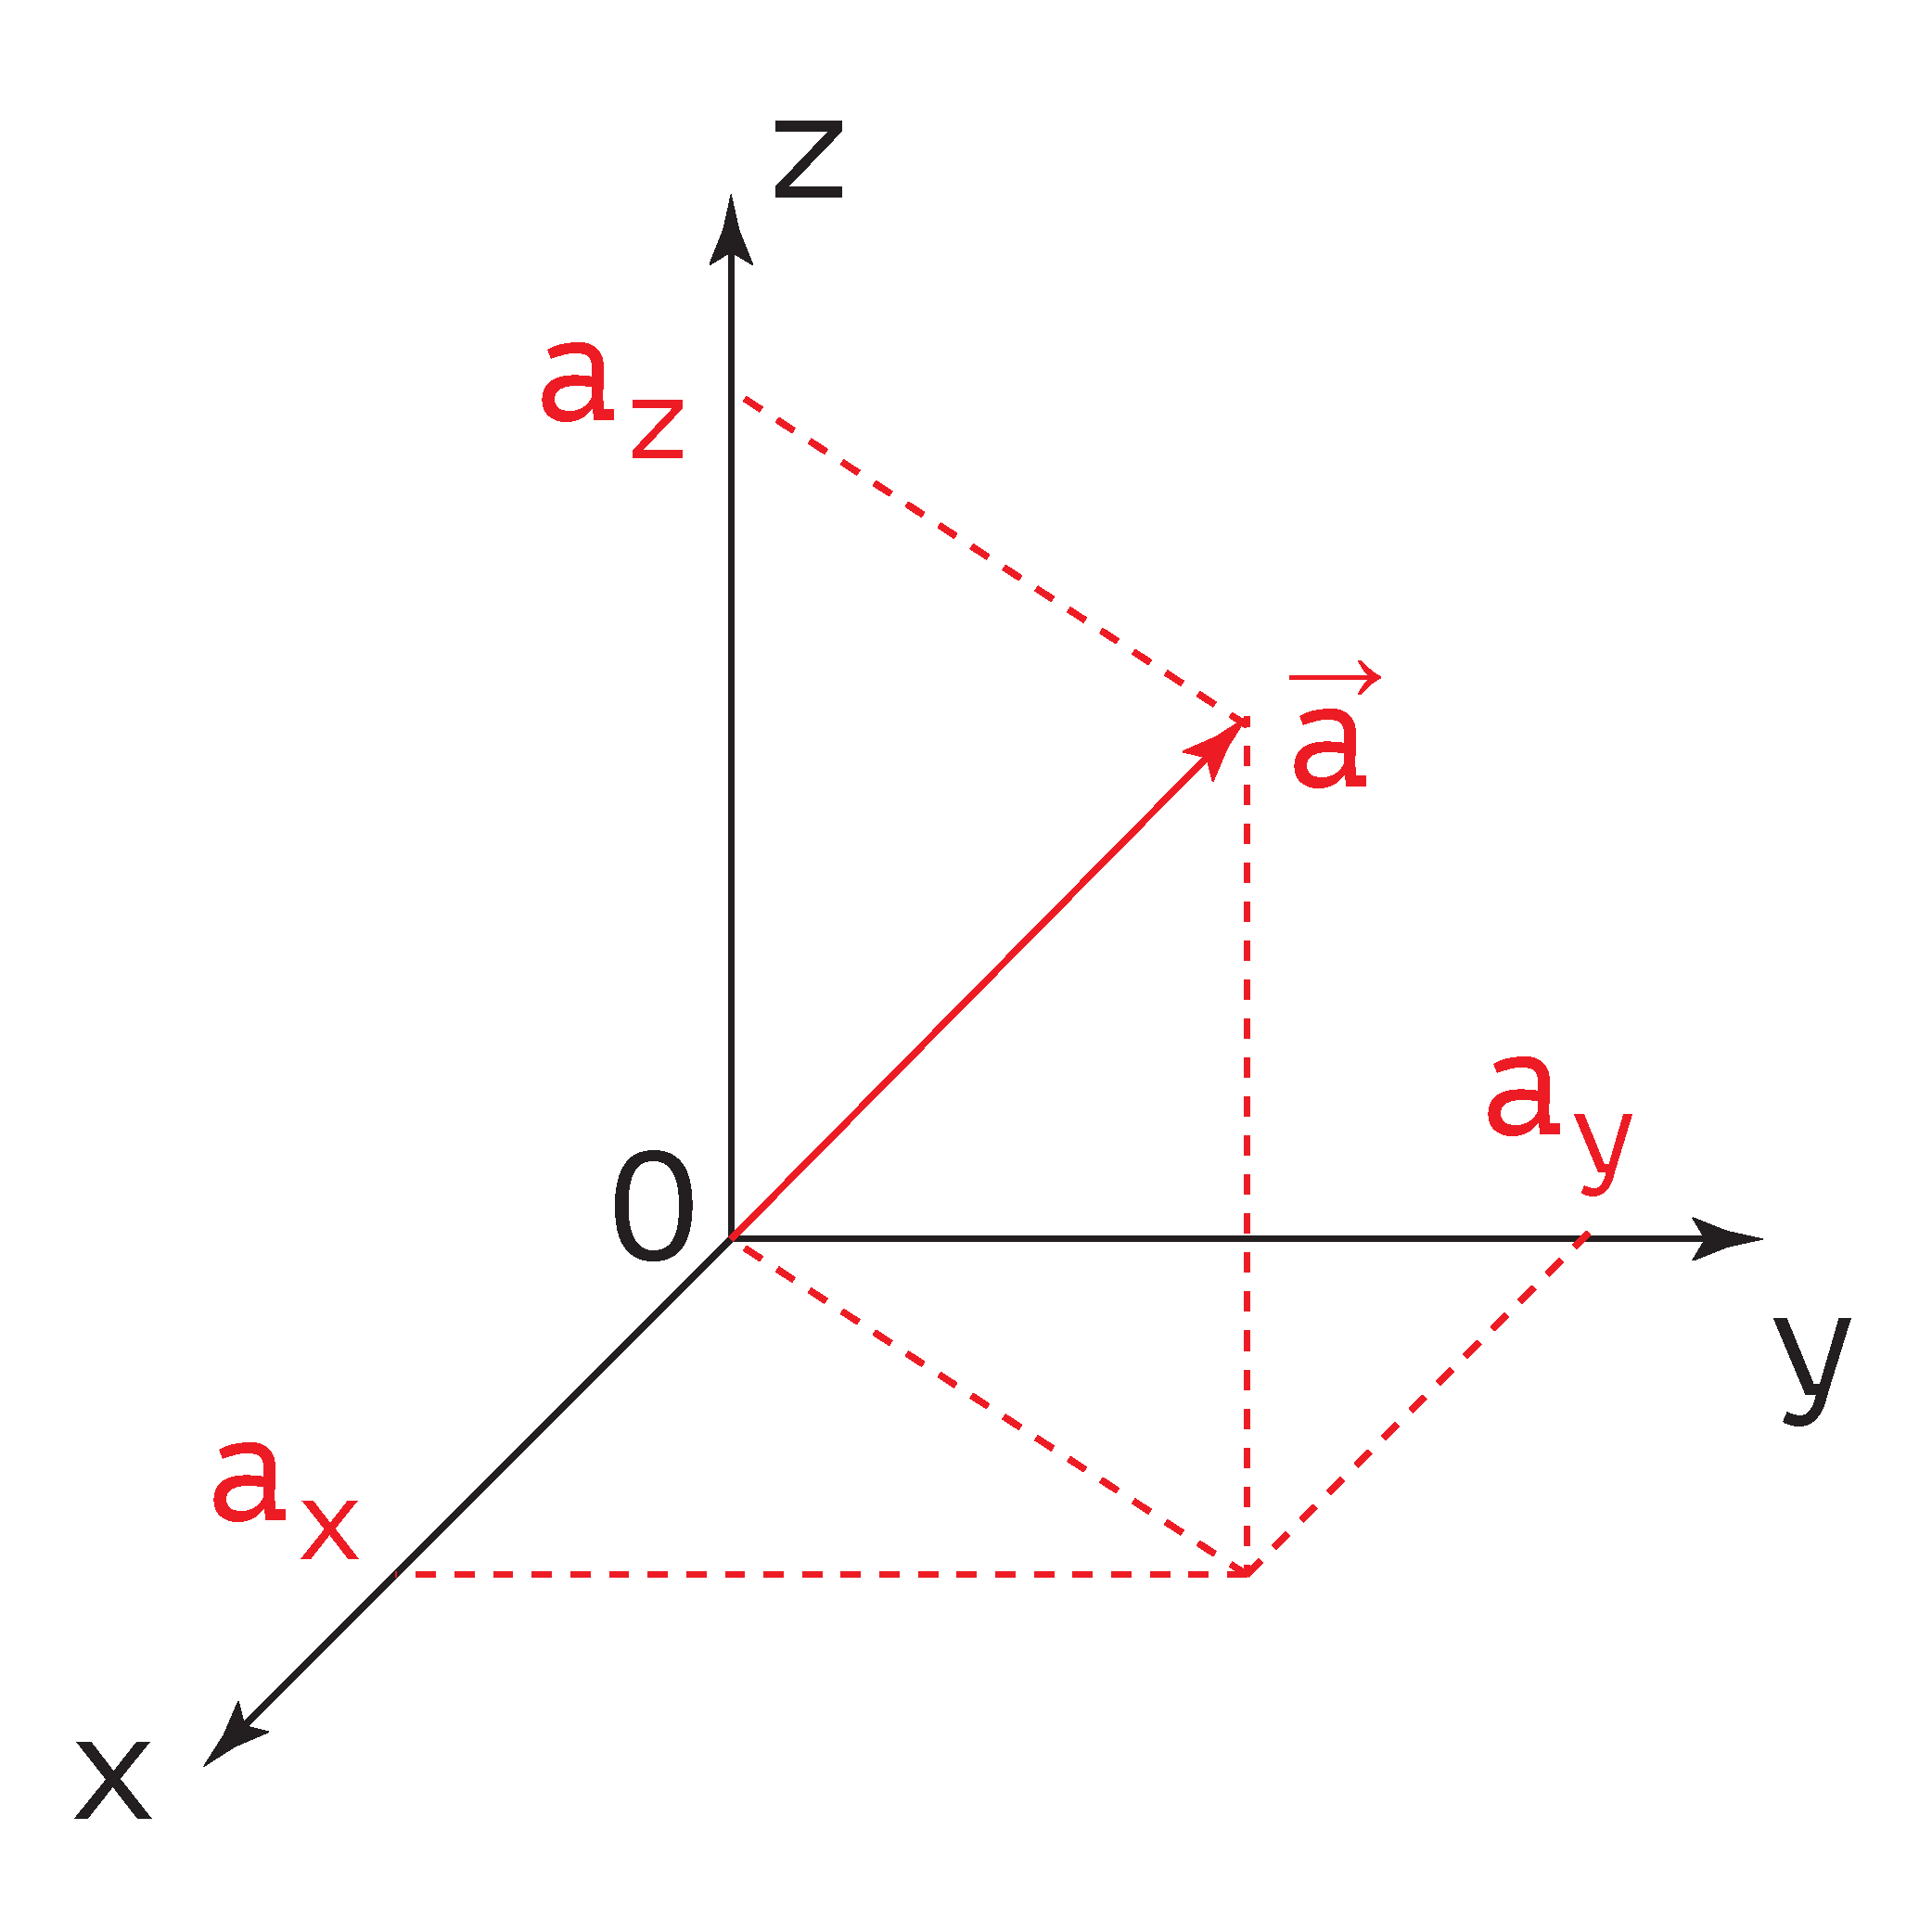
\includegraphics[width=100px]{lec01/vec_a.pdf}
    \end{figure}

    Длина этого вектора может быть найдена как \( |\vec{a}| = \sqrt{a_x^2+a_y^2+a_z^2} \). При поворотах базиса координаты вектора будут претерпевать изменения, однако, длина вектора изменяться не будет.

    \begin{definition}
        Величины или параметры, которые не изменяются при поворотах базиса, называются инвариантными относительно поворотов базиса.
    \end{definition}

    Также к инвариантам можно отнести скалярное произведение векторов \( \vec{a}\cdot\vec{b} \).
